\documentclass[12pt,a4paper,english,twoside]{book}

\usepackage[german,english]{babel}
\usepackage[T1]{fontenc}
\usepackage[utf8]{inputenc}

\usepackage{amsfonts}
\usepackage{amsmath}
\usepackage{latexsym}
\usepackage{amssymb}
\usepackage{epsfig}
\usepackage{moreverb}
\usepackage{rotating}
\usepackage{newunicodechar}
\newunicodechar{：}{:}

\usepackage{listings}
\usepackage{xcolor}
\usepackage{multirow}
\usepackage{enumerate}
\usepackage{graphics}
\usepackage{graphicx}
\graphicspath{{assets/}{./}}
\usepackage{wrapfig}
\usepackage{fancybox}
\usepackage{picinpar}
\usepackage{varioref}
\usepackage{floatflt}
\usepackage{ae}
\usepackage{textcomp}
\usepackage{float}
\usepackage{url}
\usepackage{tabularx}
\usepackage{booktabs}
\usepackage{caption}
\usepackage{siunitx}
\usepackage{hyperref}

\usepackage[
  style=numeric,
  sorting=none,
  backend=bibtex
]{biblatex}
\addbibresource{assets/refs.bib}

%\usepackage{assets/unizhdt-BA} % Bachelor Thesis
\usepackage{assets/unizhdt} % Master Thesis

%%%%%%%%%%%%%%%%%%%%%%%%%%%%%%%%%%%%%%%%%%%%%%%%%%
\newcommand{\etal}{\textit{et al}.\ }
\newcommand{\ie}{\textit{i}.\textit{e}.,\ }
\newcommand{\eg}{\textit{e}.\textit{g}.,\ }
\newcommand{\cf}{\textit{c}\textit{f}.,\ }
% Visible placeholder marker for content still to be filled in.
% Search the source for "\tbd" to find every open item.
\newcommand{\tbd}[1]{\textcolor{red}{\textbf{[TBD:} #1\textbf{]}}}
% Provisional caveat text: true as written, but flagged in red so it is easy to
% find and re-check before submission. Search the source for "\caveat".
\newcommand{\caveat}[1]{\textcolor{red}{#1}}
%%%%%%%%%%%%%%%%%%%%%%%%%%%%%%%%%%%%%%%%%%%%%%%%%%

\selectlanguage{english}
\pagestyle{headings}

\begin{document}

\lstdefinestyle{pythonstyle}{
  language=Python,
  basicstyle=\ttfamily\small,
  keywordstyle=\color{blue}\bfseries,
  commentstyle=\color{green!50!black}\itshape,
  stringstyle=\color{orange},
  numbers=left,
  numberstyle=\tiny\color{gray},
  showstringspaces=false,
  breaklines=true,
  frame=single,
  backgroundcolor=\color{gray!5},
  tabsize=4
}

\lstset{style=pythonstyle}

\author{Necati Furkan Çolak, Leyla Khasiyeva}
\authorcity{Zurich, Switzerland}
\studentid{number}
\title{Self-Explainable Graph Neural Networks via Prototype Learning for Medical Diagnosis}
\supervisors{Nasim Nezhadsistani}
\submissiondate{November 6, 2026}

\maketitle
\makeimprint

\pagenumbering{roman}

\chapter*{Declaration of Independence}


I hereby declare that I have composed this work independently and without the use of any aids other than those declared (including generative AI such as ChatGPT). I am aware that I take full responsibility for the scientific character of the submitted text myself, even if AI aids were used and declared (after written confirmation by the supervising professor). All passages taken verbatim or in sense from published or unpublished writings are identified as such. The work has not yet been submitted in the same or similar form or in excerpts as part of another examination.

\vspace{2cm}


\noindent
\begin{minipage}[t]{0.45\textwidth}
    Zürich, November 6, 2026
\end{minipage}
\hfill
\begin{minipage}[t]{0.45\textwidth}
    \raggedleft
    \rule{6cm}{0.4pt}\\[0.3cm]
    Signature of student
\end{minipage}
\chapter*{Zusammenfassung}
\addcontentsline{toc}{chapter}{Zusammenfassung}

\selectlanguage{german}

Graph Neural Networks werden zunehmend für klinische Vorhersagen aus
elektronischen Patientenakten eingesetzt, ihre Entscheidungen werden jedoch
meist erst im Nachhinein erklärt, durch Post-hoc-Attributionsverfahren, deren
Ausgabe sich nicht daran prüfen lässt, wie das Modell tatsächlich entschieden
hat. Diese Arbeit untersucht, ob eine selbsterklärende Architektur in diesem
Umfeld eine brauchbare Alternative darstellt. Aus MIMIC-IV-ED wird pro Besuch in
der Notaufnahme ein heterogener Graph gebildet, mit Vitalparametern,
Medikamenten, Symptomen und Aufnahmegrund als typisierten Knoten. Vorhergesagt
wird die Hauptdiagnose über 30 zusammengefasste Krankheitsklassen. Die
Vorhersage entsteht in einer Prototyp-Schicht, die jeden Patientengraphen mit 90
gelernten Archetypen vergleicht; diese werden auf reale Subgraphen aus den
Trainingsdaten projiziert. Das Modell wird mit einem Knowledge-Graph-GNN
(GraphCare), einer Ablation desselben Encoders ohne Prototyp-Schicht und einem
tabellarischen Gradient-Boosting-Verfahren verglichen, alle auf demselben
subjektbewussten Split.

Drei Ergebnisse stechen hervor. Das tabellarische Verfahren sagt in allen
Metriken am besten vorher (65,4\,\% Accuracy, 0,607 Macro-F1) gegenüber
56,3\,\% und 0,508 beim Prototyp-Modell. Die hier verwendete Graphstruktur
bringt also Interpretierbarkeit statt Genauigkeit. Die Prototyp-Schicht selbst
ist nahezu kostenlos: Wird sie entfernt, ändert sich die Accuracy um 0,2
Prozentpunkte. Und \caveat{bei einer Stichprobe von 50 Graphen des Test-Folds} wählen die drei
Post-hoc-Verfahren nur bei 32\,\% der Graphen denselben wichtigsten Knoten,
während die Prototyp-Evidenz in 39 dieser 50 Fälle zur Vorhersage passt und ihr
Abstand richtige von falschen Vorhersagen trennt. Das spricht dafür, die Erklärung im Modell selbst zu
verankern.

\tbd{Ein drittes Vergleichsverfahren (Methode~C) ist vorgesehen, aber noch nicht
implementiert. Sobald es vorliegt, hier einen Satz zu seinem Beitrag und seinen
Ergebnissen ergänzen und die Zahlen oben anpassen, falls sich die Reihenfolge
ändert.}

\selectlanguage{english}

\chapter*{Abstract}
\addcontentsline{toc}{chapter}{Abstract}

Graph neural networks are increasingly used for clinical prediction from
electronic health records, but they are usually explained after the fact, by
post-hoc attribution methods whose output cannot be checked against the way the
model actually decided. This project asks whether a self-explainable
architecture is a workable alternative in that setting. We build one
heterogeneous graph per emergency-department visit from MIMIC-IV-ED, with
vital signs, medications, symptoms and chief complaints as typed nodes, and
predict the primary diagnosis across 30 merged disease classes. Predictions are
made by a prototype layer that compares each patient graph to 90 learned
archetypes, which are projected onto real training subgraphs. The model is
compared against a knowledge-graph GNN (GraphCare), a prototype-free ablation of
the same encoder, and a tabular gradient-boosting baseline, all on one canonical
subject-aware split.

Three results stand out. The tabular baseline is the strongest predictor on
every metric (65.4\% accuracy, 0.607 macro-F1) against 56.3\% and 0.508 for the
prototype model, so the graph structure used here adds interpretability rather
than accuracy. The prototype layer itself is close to free: removing it changes
accuracy by 0.2 percentage points. And \caveat{on a 50-graph sample of the test fold}, the three post-hoc
explainers agree on the most important node in only
32\% of the cases, while the prototype evidence matches the prediction in 39 of
those 50 and its distance separates correct from incorrect predictions, which
argues for building the explanation into the model.

\tbd{A third comparison method (Method~C) is planned but not yet implemented.
Once it is, add one sentence here describing what it contributes and how it
scores, and update the numbers above if it changes the ordering.}

\chapter*{Acknowledgments}
\addcontentsline{toc}{chapter}{Acknowledgments}

As this project nears completion, we would like to express our sincere gratitude to our supervisor, Nasim Nezhadsistani. Throughout the research and writing process, Nasim provided us with extremely patient and invaluable guidance, from the conception of the research topic to the refinement of the research details.

We would also like to thank Prof.~Dr.~Burkhard Stiller for allowing us to complete this project in the Communication Systems Group and for his advice throughout the process.

\tableofcontents

\cleardoublepage
\pagenumbering{arabic}

\chapter{Introduction}\label{introduction}

\section{Motivation}
The digitization of healthcare has led to the widespread use of Electronic Health Records, which are inherently heterogeneous, high-dimensional, and longitudinal. These characteristics make clinical risk prediction particularly challenging~\cite{ossboll2024gnn}. In recent years, Graph Neural Networks have emerged as a promising approach in this domain, since representing patients as graphs of medical entities allows them to capture relational and temporal structures that traditional models often fail to model effectively~\cite{ossboll2024gnn,mesinovic2026dynagraph}.

Despite their strong predimctive performance, GNNs still suffer from an important limitation: they remain largely black box models. As noted in prior work, ``a major limitation of deep models is that they are not amenable to interpretability''~\cite{yuan2022explainability}. In clinical settings, where transparency is essential for trust and medical decision making, this lack of interpretability is especially problematic.

Most existing work addresses this issue using post-hoc explanation methods such as GNNExplainer~\cite{ying2019gnnexplainer}. However, these methods are applied after the model has already made its prediction, which makes it unclear whether the explanations truly reflect how the model arrived at its decision. In addition, their performance can be inconsistent when applied to larger datasets or more complex evaluation settings~\cite{agarwal2023graphxai}.

An alternative approach is using methods with built-in interpretability whose internal decision-making logic is transparent and directly explainable to humans. One of such methods is ProtGNN, which is a prototype-based model that explains its decisions by comparing a test instance to learned representative cases, driving predictions based on similarities ~\cite{zhang2022protgnn}. However, most work on this type of model has been tested on molecular data, so it is still unclear how well it works for healthcare applications. The closest related work in this area, ProtoEHR, applies a similar idea to Electronic Health Records data, but it does not identify which parts of the patient graph drive the prediction and does not compare its explanations with post-hoc methods in a consistent way~\cite{cai2025protoehr}.

This project aims to address this gap by developing a self-explainable GNN for EHR-based diagnosis that incorporates a built-in explainable layer. Three models were implemented on the same patient dataset, where each model is designed to make predictions and to extract the medical subgraph that drives each of those predictions, specifically through prototype matching, internal attention mechanisms, or 3RD METHOD'S APPROACH. Each approach will be evaluated in terms of both predictive performance and explanation quality, and compared against post-hoc baselines using the GraphXAI framework~\cite{agarwal2023graphxai}.

\section{Description of Work}
This Master's project is structured in three phases. First, a focused literature review will be conducted on GNN-based clinical prediction from EHR data, post-hoc explanation methods and their limitations, and different methods with built-in interpretability.

Second, an EHR-to-graph pipeline will be developed using the MIMIC-IV-ED dataset~\cite{johnson2023mimicived}. Medical entities such as diagnoses, medications, lab results, and procedures will be represented as nodes, while edges will capture temporal and clinical relationships. To achieve interpretability, built-in explainability layers will be embedded into the graph neural network architectures to identify clinical patterns in predictions and highlight the most relevant medical subgraphs.

Third, the model will be evaluated along two dimensions. Predictive performance will be measured with multi-class metrics and compared against a tabular baseline and other GNN methods trained on the same split. Explanation quality will be assessed with sparsity and inter-explainer agreement, and compared with post-hoc methods within the GraphXAI framework~\cite{agarwal2023graphxai}.

The project aims to provide a reproducible self-explainable GNN framework for EHR-based diagnosis, documented in a report aligned with scientific research standards.

\chapter{Project Outline}

This chapter should define the scope, objectives, research questions, methodology, expected contributions, and organization of the project.

\textbf{RQ1}: How does the proposed prototype-based self-explainable GNN perform compared with tabular, standard GNN, and knowledge-graph baselines for imbalanced multi-class diagnosis?

\textbf{RQ2}: What is the contribution of the prototype layer and prototype-projection mechanism to predictive performance and interpretability?

\textbf{RQ3}: How faithful, stable, sparse, and clinically meaningful are the intrinsic and post-hoc explanations generated by the proposed approach?


\chapter{Background}\label{background}

This chapter presents the technical foundations underlying this project.
Section~\ref{sec:gnn} introduces Graph Neural Networks (GNNs) and the
message-passing paradigm. Section~\ref{sec:gnn-ehr} reviews the application of
GNNs to Electronic Health Records (EHRs) for clinical risk prediction.
Section~\ref{sec:what-is-xai} introduces Explainable AI and the
interpretability--performance trade-off in the clinical context.
Section~\ref{sec:xai-gnn} discusses explainability in GNNs and highlights the
limitations of post-hoc approaches. Finally, Section~\ref{sec:proto} introduces
prototype learning as an inherently interpretable alternative.

%===============================================================
\section{Graph Neural Networks}
\label{sec:gnn}
%===============================================================

A graph is defined as $G = (V, E)$, where $V$ denotes the set of nodes and
$E \subseteq V \times V$ represents the set of edges. Each node $v \in V$ is
associated with a feature vector $\mathbf{x}_v \in \mathbb{R}^d$, and edges may
also carry features. Graph Neural Networks (GNNs) are deep learning models
designed to learn representations of nodes, edges, or entire graphs by
exploiting the underlying graph structure~\cite{yuan2022explainability}.

The core mechanism of GNNs is \emph{message passing}. At layer $k$, each node
updates its representation by aggregating information from its neighbours
$\mathcal{N}(v)$:
%
\begin{equation}
\mathbf{h}_v^{(k+1)} = \sigma\!\left(
  \sum_{u \in \mathcal{N}(v) \cup \{v\}}
  \tilde{\mathbf{A}}_{uv}\, \mathbf{W}^{(k)} \mathbf{h}_u^{(k)}
\right),
\end{equation}
%
where $\mathbf{W}^{(k)}$ is a learnable weight matrix, $\tilde{\mathbf{A}}$ is
the normalised adjacency matrix including self-loops, and $\sigma(\cdot)$ is a
non-linear activation function~\cite{kipf2017gcn}. After $L$ layers, node
embeddings capture information from their $L$-hop neighbourhoods. For
graph-level tasks, a readout function (e.g.\ mean, max, or sum pooling)
aggregates node embeddings into a single graph representation $\mathbf{h}_G$.

In this work we build on two widely used GNN architectures. The Graph
Convolutional Network (GCN)~\cite{kipf2017gcn} applies symmetric normalisation
to the adjacency matrix during aggregation and serves as the encoder of our
model. The Graph Attention Network (GAT)~\cite{velickovic2018gat} instead
learns attention weights that assign different importance to neighbouring
nodes, which is useful in clinical settings where the relevance of relations
between entities may vary~\cite{ossboll2024gnn}; it is implemented as an
alternative encoder for comparison.

%===============================================================
\section{Graph Neural Networks for Electronic Health Records}
\label{sec:gnn-ehr}
%===============================================================

EHRs are inherently relational: a single emergency-department visit links a
patient to diagnoses, medications, laboratory results, procedures, and vital
signs, and a patient accumulates many such visits over time. This structure
makes GNNs a natural fit for clinical prediction, and a growing body of work
applies them to tasks such as mortality prediction, readmission, and
diagnosis~\cite{ossboll2024gnn}.

Two graph-construction paradigms dominate. In the first, \emph{population} (or
\emph{patient-similarity}) graphs, each patient is a node and edges connect
clinically similar patients, so that label information can propagate between
comparable cases. In the second, \emph{intra-patient} graphs, the medical
entities of a visit (diagnoses, medications, vitals) become nodes and edges
encode their clinical relationships; prediction is then a graph-classification
task with one graph per patient. The latter yields a topology that is
clinically meaningful rather than a pure similarity heuristic, and it is the
formulation adopted in this work (Chapter~\ref{architecture}).

Several methods build on these paradigms. Temporal approaches such as DynaGraph
model the sequence of visits as a dynamic graph to capture disease
progression~\cite{mesinovic2026dynagraph}. GraphCare follows a knowledge-graph
route and serves as the main GNN comparison baseline in this project; it is
described in Section~\ref{sec:graphcare}. Most of these models remain black
boxes: they predict accurately but do not expose which entities or relations
drove a decision. ProtoEHR is the closest prior work to ours: it brings
prototype-based, case-based reasoning to hierarchical EHR data, but it does not
identify which parts of the patient graph drive each prediction, nor does it
compare its explanations against post-hoc methods~\cite{cai2025protoehr}.

%===============================================================
\section{Explainable Artificial Intelligence (XAI)}
\label{sec:what-is-xai}
%===============================================================

As Artificial Intelligence (AI) systems are increasingly integrated into
critical domains like healthcare, the ``black-box'' nature of deep learning
models has become a primary barrier to adoption. Explainable AI (XAI) refers to
machine learning techniques designed to make the predictions of AI models
understandable to human experts~\cite{yuan2022explainability}.

\subsection{The Interpretability--Performance Trade-off}\label{sec:tradeoff}

Historically, it was assumed that there exists a trade-off between model
complexity (performance) and interpretability. Simple models, such as linear
regression or decision trees, are more intuitive and interpretable but often
fail to capture the complex, non-linear dependencies found in multi-modal EHR
data. Conversely, GNNs hold high predictive power but fail to provide insight
into \emph{how and why} a specific outcome was reached. XAI seeks to resolve
this either by creating post-hoc tools to probe complex models or by designing
``interpretable-by-design'' architectures.

\subsection{XAI in the Clinical Context}

In healthcare, interpretability has become a requirement for safety and
accountability. Clinical XAI must satisfy the ``right to explanation'' under
legal frameworks like the GDPR and provide practitioners with actionable and
reliable evidence. For instance, an explainer that highlights a patient's age
as the primary risk factor for a disease is less clinically useful than one
that highlights a specific combination of rising creatinine levels and falling
blood pressure.

%===============================================================
\section{Explainability in Graph Neural Networks}
\label{sec:xai-gnn}
%===============================================================

Despite their strong predictive performance, GNNs are often considered
black-box models. Existing explainability methods can be broadly categorised
into instance-level and model-level approaches~\cite{yuan2022explainability}.
Instance-level methods aim to explain individual predictions and can be further
divided into gradient-based, perturbation-based, decomposition-based, and
surrogate-based techniques.

A common characteristic of these methods is that they are \emph{post-hoc}: they
attempt to explain a trained model after the prediction has been made.
Typically, they identify a subgraph that maximises the mutual information with
the model's output. However, this design introduces two key limitations. First,
explanations are not guaranteed to reflect the true reasoning of the model,
since the explanation mechanism is separate from the prediction
process~\cite{zhang2022protgnn}. Second, large-scale evaluations such as
GraphXAI show that many post-hoc methods struggle with large or complex
explanations and may fail to preserve fairness properties, both of which are
critical in clinical applications~\cite{agarwal2023graphxai}.

To evaluate explainability methods, the literature relies on metrics such as
fidelity, accuracy, stability, and sparsity~\cite{agarwal2023graphxai}. Because
the clinical data in this project has no ground-truth importance masks,
explanation quality is assessed primarily through sparsity, inter-explainer
agreement, and, optionally, fidelity, while ground-truth-dependent metrics
such as explanation accuracy are not applicable
(Chapter~\ref{implementation}).

%===============================================================
\section{Prototype Learning and Case-Based Reasoning}
\label{sec:proto}
%===============================================================

Prototype learning is inspired by \emph{case-based reasoning}, where new
instances are classified by comparing them to representative examples. In deep
learning, this idea was popularised by ProtoPNet, which introduces a prototype
layer that stores representative patterns and classifies inputs based on their
similarity to these prototypes~\cite{chen2019protopnet}.

This concept has been extended to graph data through ProtGNN. The model consists
of three components: a GNN encoder $f$ that produces a graph embedding
$\mathbf{h}$, a prototype layer $g_P$ containing $K$ learnable prototype vectors
$\{\mathbf{p}_j\}$, and a final classification layer~\cite{zhang2022protgnn}.
The similarity between an embedding and a prototype is computed as
%
\begin{equation}
\mathrm{sim}(\mathbf{p}_k, \mathbf{h}) = \log\!\left(
  \frac{\lVert \mathbf{p}_k - \mathbf{h}\rVert_2^2 + 1}
       {\lVert \mathbf{p}_k - \mathbf{h}\rVert_2^2 + \epsilon}
\right),
\end{equation}
%
which yields a positive, distance-based similarity score that is maximal when
the embedding coincides with the prototype and decays towards zero as the
distance grows.

The training objective combines a classification loss with regularisation terms
that shape the prototype space: a cluster loss (encouraging embeddings to be
close to same-class prototypes), a separation loss (pushing embeddings away from
other-class prototypes), and, in the original ProtGNN, a diversity loss
(preventing prototype collapse)~\cite{zhang2022protgnn}. The clinical adaptation
used in this project retains the cluster and separation terms but replaces the
diversity term with an $\ell_1$ sparsity penalty on the classification layer
(Chapter~\ref{implementation}).

A key feature of prototype learning is \emph{prototype projection}, where each
prototype is periodically aligned with the closest real training example. In
ProtGNN, this is achieved using Monte Carlo Tree Search (MCTS) to efficiently
explore the space of possible subgraphs~\cite{zhang2022protgnn}. Unlike post-hoc
methods, prototype-based models provide explanations as part of the prediction
process itself, making them inherently interpretable. In the clinical domain,
ProtoEHR extends this idea to hierarchical EHR data, making it the closest prior
work to this project~\cite{cai2025protoehr}.

%===============================================================
\section{Knowledge-Graph GNNs and GraphCare}
\label{sec:graphcare}
%===============================================================

Prototype models represent one route to interpretable EHR prediction. A second
route enriches the patient graph with external medical knowledge before a GNN is
applied. GraphCare is the representative method of this route and serves as the
main GNN comparison baseline in this project~\cite{jiang2024graphcare}.

GraphCare builds a personalised knowledge graph for each patient. Rather than
relying only on the relations present in the dataset, it extracts relational
knowledge about medical concepts from large language models and from external
biomedical knowledge bases, and attaches it to the patient's diagnoses,
procedures, and medications. The result is a patient-specific graph that carries
context a raw record does not contain.

Prediction is performed by a Bi-attention Augmented (BAT) graph neural network.
The bi-attention mechanism weights both the nodes of the personalised graph and
the visits over time, so the model can focus on the concepts and moments most
relevant to a given prediction. In the original work, GraphCare was evaluated on
MIMIC-III and MIMIC-IV across mortality prediction, readmission, length of stay,
and drug recommendation, and reported its largest gains in settings with limited
training data.

Two properties matter for this project. GraphCare and the proposed prototype
model share the same graph-classification setting, which makes a controlled
comparison on the same split meaningful. Their interpretability differs in kind:
GraphCare exposes attention weights over the personalised graph, whereas the
prototype model explains a prediction through similarity to learned cases and
through node attribution over the patient graph. This difference is the reason
GraphCare is used as the reference point in the evaluation
(Chapter~\ref{evaluation}).

\section{Method 3}
\label{sec:method3}
\chapter{Related Work}\label{relatedwork}

This project sits at the intersection of three lines of research: graph neural
networks for clinical prediction from EHR data, explainability methods for GNNs,
and intrinsicly explainable models that build interpretability into the prediction itself. This chapter reviews each line and then positions the proposed model
against the closest prior work.

\section{Graph Neural Networks for EHR Prediction}

A patient record is relational by nature. A single visit ties a patient to
diagnoses, medications, laboratory results, and vital signs, and a patient
accumulates many such visits over time. This rich and heterogeneous structure has made GNNs a common
choice for clinical prediction, and a recent survey catalogues their use across
mortality prediction, readmission, and diagnosis~\cite{ossboll2024gnn}.

The reviewed work differs mainly in how the graph is built and whether time is
modelled. DynaGraph learns a dynamic graph over the sequence of visits and uses
visit-level attention to capture disease progression, reporting gains over a
range of baselines on ICU cohorts~\cite{mesinovic2026dynagraph}. GraphCare takes
a different route: it extracts a personalised knowledge graph for each patient
from large language models and external biomedical knowledge bases, then trains
a bi-attention graph network on the resulting structure~\cite{jiang2024graphcare}.
Both inject or learn structure beyond the raw record, and both report attention
weights as a form of interpretability. However, neither model extracts a concrete, minimal subgraph that drove the prediction, which is the level of explanation a clinician needs to verify a conclusion of a classifier model. 

\section{Explainability in Graph Neural Networks}

Because the mechanism of most GNNs remain ambiguous, a separate body of work develops methods to
explain them after training. A taxonomic survey groups these post-hoc methods
into instance-level and model-level approaches, with instance-level techniques further split into gradient-based, perturbation-based, decomposition-based, and surrogate families~\cite{yuan2022explainability}. GNNExplainer is a widely used instance-level method that learns an edge mask maximizing mutual information
with the prediction.

Two problems limit these methods in a clinical setting. The explanation is
produced by a mechanism separate from the model, so it is not guaranteed to
accurately reflect the reasoning that led to the prediction. Their behaviour is also
uneven: the GraphXAI benchmark introduces a synthetic generator with
ground-truth importance masks and four evaluation metrics, and shows that many
post-hoc explainers degrade on larger or denser graphs and can fail to preserve
fairness properties~\cite{agarwal2023graphxai}. This project uses the same
GraphXAI framework, but applies it to compare inherent explainability layers of the chosen models on real clinical graphs where no ground-truth mask exists.

\section{Prototype-Based Self-Explaining Models}

An alternative to post-hoc explanation is to make the model interpretable by
construction. Prototype learning follows case-based reasoning: a new input is
classified by comparing it to a set of learned representative examples. ProtoPNet
introduced this idea for image recognition with a prototype layer, and ProtGNN
extended it to graphs, using a Monte Carlo Tree Search to project each prototype
onto a real subgraph~\cite{zhang2022protgnn}. ProtGNN was evaluated on molecular
datasets such as MUTAG, so its behaviour on clinical data was left open.

ProtoEHR is the closest prior work to this project. It brings hierarchical
prototype learning to EHR data, organising prototypes at the code, visit, and
patient levels~\cite{cai2025protoehr}. Two gaps remain. ProtoEHR does not
identify which parts of a patient graph drive a prediction, and it does not
compare its built-in explanations against post-hoc methods. The model proposed
here targets both gaps by pairing a prototype layer with GraphXAI node attribution on intra-patient graphs.

\section{Positioning}

Table~\ref{tab:positioning} places the proposed models against their closest
methods. The combination that distinguishes this work is a prototype-based
classifier over intra-patient EHR graphs that also produces node-level
explanations and evaluates them against post-hoc explainers on the same data.

\begin{table}[htbp]
  \centering
  \small
  \caption{Positioning of the proposed model against the closest prior work.}
  \label{tab:positioning}
  \begin{tabular}{lllcc}
    \toprule
    Method & Interpretability & Domain & Node-level & Post-hoc \\
           & style            &        & explanation & comparison \\
    \midrule
    ProtGNN~\cite{zhang2022protgnn}        & Prototypes            & Molecular & Subgraph & No \\
    ProtoEHR~\cite{cai2025protoehr}        & Hierarchical prot.\   & EHR       & No       & No \\
    GraphCare~\cite{jiang2024graphcare}    & Bi-attention (KG)     & EHR       & No       & No \\
    DynaGraph~\cite{mesinovic2026dynagraph}& Visit attention       & EHR (ICU) & No       & No \\
    Method~C \tbd{name}                    & \tbd{}                & \tbd{}    & \tbd{}   & \tbd{} \\
    This work                              & Prototypes            & EHR (ED)  & Yes      & Yes \\
    \bottomrule
  \end{tabular}
\end{table}

The prototype family (ProtGNN, ProtoEHR) provides case-based reasoning but stops
short of pointing to the clinical entities behind a decision. The attention-based
EHR models (GraphCare, DynaGraph) expose attention weights but were not built to
compare those weights against independent post-hoc explainers. By combining a
prototype layer with GraphXAI node attribution on intra-patient graphs, this
project addresses the gap left by both groups.

\chapter{Architecture}\label{architecture}
This chapter describes the architectures of the three methods compared in this project. All three address the same task, the 30-class emergency-department diagnosis introduced in Chapter~\ref{implementation}, and are trained and evaluated on the same cohort and split. They differ in how they represent a patient and how they reach an interpretable prediction. Section~\ref{sec:shared-framework} sets out the common ground. The prototype-based model is described in Section~\ref{sec:pillar-protgnn}, the knowledge-graph model GraphCare in Section~\ref{sec:pillar-graphcare}, and the third method in Section~\ref{sec:pillar-methodc}.

\section{Shared Framework}\label{sec:shared-framework}
The three methods share the parts of the problem that make their comparison controlled. Each predicts the primary diagnosis of an emergency-department visit as one of 30 classes. Each is trained on the same MIMIC-IV-ED cohort under the same subject-aware split, so no patient appears in more than one fold. Each draws on the same underlying clinical signal: the diagnosis, medication, and symptom vocabulary together with the population-level PMI co-occurrence statistics between medications.

What differs is the graph. The prototype-based model builds one intra-patient graph per visit and classifies it directly. GraphCare reasons over a personalised knowledge graph assembled from an ontology and external knowledge. The third method adds a further representation, described in Section~\ref{sec:pillar-methodc}. Each of the following sections describes one of these designs in full.

\section{Prototype-Based Model (ProtGNN)}\label{sec:pillar-protgnn}
This method follows a four-stage pipeline that transforms raw clinical records into interpretable diagnostic insights.

\subsection{Conceptual Data Flow}

\begin{enumerate}
  \item \textbf{Graph Construction (EHR to Graph).} Tabular patient records from the MIMIC-IV Emergency Department module are converted into intra-patient heterogeneous graphs. Each patient becomes its own graph, where the patient node is central, and is connected to clinical entity nodes. Out of these clinical entity nodes, there is one node per vital sign measurement, one node per taken medication, one node per symptom recorded by the attending clinician, and one for the chief complaint recorded at triage. Additionally, medications that frequently co-occur among the patients are linked via direct edges, which are derived from Pointwise Mutual Information (PMI) scores. As a result, a clinical visit becomes a relational structure: the graph encodes both the patient's individual clinical findings and the relations between co-occurring clinical entities.

  \item \textbf{GNN Encoder.}
        The patient graph is processed through a multi-layer Graph Convolutional Network (GCN). Through the message-passing paradigm, the encoder aggregates neighbourhood information across node types into a single graph-level embedding $\mathbf{h}_G \in \mathbb{R}^{d}$ via global mean pooling. The GCN propagates information from medication nodes via PMI co-occurrence edges, where drug-bundle patterns of co-occurrence (e.g.\
        the Cardiac bundle: Aspirin - metoprolol - atorvastatin - lisinopril) influence the final embedding.

  \item \textbf{The Prototype Layer.}
        The embedding $\mathbf{h}_G$ is projected into a \textit{Prototype Space} containing $K$ learned disease prototypes $\{\mathbf{p}_k\}_{k=1}^{K}$. Each prototype is a vector in the same latent space as $\mathbf{h}_G$,
        trained to represent a typical clinical profile for one of the 30 disease classes. The model computes a log-distance similarity score between the patient embedding and every prototype. This produces a set of case-based reasoning scores that
        contribute to the final prediction. This makes the model's logic analogous to clinical pattern recognition: a patient is classified as having heart failure because its graph embedding lies close to prototypes learned from other heart-failure patients.

  \item \textbf{Dual Output: Prediction and Explanation.}
        The final stage produces two outputs at once. The classification output is a probability distribution over 30 disease classes, derived as a linear combination of the prototype similarity scores. The explanation output is a node importance vector produced by a GraphXAI explainer, which identifies which clinical entity nodes in the patient
        graph contributed most to the prediction: vital signs, medications, symptoms, or chief complaints. Together these outputs answer both \textit{what} the model predicts and \textit{why}.
\end{enumerate}

\begin{figure}[htbp]
    \centering
    % \includegraphics[width=\textwidth]{assets/architecture_diagram.pdf}
    \caption{Overview of the prototype-based model. Patient EHR records are converted to intra-patient heterogeneous graphs, encoded by a GCN, compared
             against learned prototypes, and explained by a GraphXAI explainer.}
    \label{fig:framework_diagram}
\end{figure}

\subsection{Input Layer and Graph Formulation}

Each patient record is formulated as a graph $G = (V, E)$ whose node
set $V$ consists of five typed subsets:

\begin{itemize}
  \item \textbf{Patient} node (index~0) encodes demographics, transport mode, medical history flags, lab value summaries, medication class counts, and vital sign trend statistics (min, max, standard deviation across the visit).
  \item $|V_\text{vital}| = 15$ \textbf{Vital} nodes, one for each monitored vital sign (temperature, heart rate, respiratory rate, oxygen saturation, systolic and diastolic blood pressure, pain score, acuity, and eight triage vital-sign statistics). Each vital node encodes a z-scored measurement value, an abnormality flag ($|z| > 2$), and a missingness flag.
  \item $|V_\text{med}|$ \textbf{Medication} nodes, one for each medication taken by the given patient, which has been assigned to more than a threshold of $1\%$ of the population, covering both home medications and ED-dispensed drugs.
  \item $|V_\text{sym}|$ \textbf{Symptom} nodes, one for each ICD-coded symptom recorded by the clinician at triage.
  \item $|V_\text{cc}|$ \textbf{Chief Complaint} nodes, one per complaint recorded at triage.
\end{itemize}

The edge set $E$ contains two bidirectional types of connections:

\begin{itemize}
  \item \textbf{Patient-entity edges}: the Patient node connects to every vital, medication, symptom, and chief complaint node it is associated with.
  \item \textbf{Medication--medication PMI edges}: to encode clinically meaningful drug co-occurrence patterns, any two medication nodes whose population-level PMI score exceeds a threshold of $2.0$ are directly connected with an edge  (e.g.\ the cardiac bundle, the asthma bundle).
\end{itemize}

Every node, regardless of type, carries the same $D$-dimensional feature vector (where $D = 415$ in the full disease dataset). The feature layout is fixed: a 6-slot type one-hot block (one slot is reserved for ICD nodes and stays unused in the disease setting), followed by identity blocks for each node type vocabulary (vital identity, medication identity, symptom identity, chief complaint identity), a scalar value slot, abnormality and missingness flags, a demographics block, and a patient numeric block. Only the slots corresponding to a node's own type are populated, and all others are set to zero. This uniform feature dimension is required for the weight-sharing across node types in the GCN.

\subsection{GNN Encoder $f$}

The encoder $f: G \rightarrow \mathbf{h}_G$ is a three-layer GCN with hidden dimensions $[128, 128, 128]$ and ReLU nonlinearities:
\[
  \mathbf{H}^{(\ell)} = \sigma\!\left(
    \tilde{D}^{-1/2}\tilde{A}\tilde{D}^{-1/2}
    \mathbf{H}^{(\ell-1)} W^{(\ell)}
  \right), \quad \ell = 1, 2, 3,
\]
where $\tilde{A} = A + I$ is the adjacency matrix with self-loops, $\tilde{D}$ is its degree matrix, $W^{(\ell)}$ are learnable weights, and $\sigma$ is ReLU. Dropout ($p = 0.51$) is applied after each layer. The graph-level representation is obtained by global mean pooling:
\[
  \mathbf{h}_G = \frac{1}{|V|}\sum_{v \in V} \mathbf{H}^{(3)}_v.
\]

A single 64-dimensional MLP hidden layer followed by a linear output layer maps $\mathbf{h}_G$ to class logits when prototype layers are disabled.

\subsection{Prototype Matching and Latent Similarity $g_P$}

The Prototype Layer $g_P$ maintains $K = C \times m$ learnable prototype vectors $\{\mathbf{p}_k\}$, where $C = 30$ is the number of disease classes and $m = 3$ is the number of prototypes per class, for a total of $K = 90$ prototypes. The similarity between the patient embedding and each prototype is computed as:
\[
  \mathrm{sim}(\mathbf{h}_G, \mathbf{p}_k)
  = \log\!\left(
      \frac{\|\mathbf{h}_G - \mathbf{p}_k\|_2^2 + 1}
           {\|\mathbf{h}_G - \mathbf{p}_k\|_2^2 + \varepsilon}
    \right),
\]
with $\varepsilon = 10^{-4}$. This formulation maps distance monotonically to similarity: the score is maximal when the patient embedding coincides with the prototype and decays toward zero as the distance grows. The final logits are $\hat{\mathbf{y}} = W_{\mathrm{last}}\, \boldsymbol{s}$, where $\boldsymbol{s} \in \mathbb{R}^{90}$ collects all similarity scores. $W_{\mathrm{last}}$ is a linear layer initialised to encode class-prototype membership and fine-tuned during joint training (Chapter~\ref{implementation}).

Training optimizes a composite loss:
\[
  \mathcal{L} = \mathcal{L}_{\mathrm{CE}}
              + \lambda_c \mathcal{L}_{\mathrm{cluster}}
              + \lambda_s \mathcal{L}_{\mathrm{sep}}
              + \lambda_\ell \|\mathbf{W}_{\mathrm{last}}
                               \odot M_\perp\|_1,
\]
which consists of cross-entropy $\mathcal{L}_{\mathrm{CE}}$, along with $\mathcal{L}_{\mathrm{cluster}}$ loss, which brings each embedding closer towards its closest same-class prototype, a margin-based cost $\mathcal{L}_{\mathrm{sep}}$ that penalizes wrong-class prototypes, activated only when closer than a margin threshold (bounded in $[0, \text{margin}]$ per sample for numerical stability), and the $\ell_1$ term, which penalizes cross-class weights in the last layer.

Periodically, prototype vectors are projected onto real patient subgraphs via a Monte Carlo Tree Search (MCTS) procedure. This procedure ensures that each prototype corresponds to an actual clinical substructure rather than an abstract latent point.

\subsection{GraphXAI Explanation Module}

Explanations are generated using three complementary GraphXAI
explainers~\cite{agarwal2023graphxai}, each producing a node importance vector:

\begin{itemize}
  \item \textbf{GradExplainer} attributes importance by backpropagating the prediction loss to node features and summing absolute gradient magnitudes per node.

  \item \textbf{IntegratedGradExplainer} integrates gradients along a path from a zero baseline to the input, reducing noise from local gradient saturation and providing attribution with provable completeness.

  \item \textbf{GNNExplainer} learns a soft mask over edges by maximizing mutual information between the masked subgraph and the model prediction. Node importance is derived from the learned edge mask.
\end{itemize}

When prototype layers are active, the explainers are routed through a specialized architecture wrapper to handle the models' inherent interpretability layers. For instance, when analyzing models with highly nonlinear or distance-based components, this wrapper safely routes gradients directly to the underlying GNN backbone. This is a necessary step, because otherwise, the log-distance similarity formula suppresses gradient magnitudes by two orders of magnitude, rendering gradient-based explainers ineffective. By optimizing this routing for each model, the explainers can consistently produce meaningful attribution scores across all architectures.

The top-$k$ nodes identified by each explainer make up the explanation of the model. In the clinical setting, these
explanation nodes correspond to readings of vital signs, medications, symptoms, or chief complaints that led to the disease prediction. This provides clinicians with a clear and inspectable justification for the model's output.

\section{Knowledge-Graph Model (GraphCare)}\label{sec:pillar-graphcare}

The second method, GraphCare, reaches an interpretable prediction through a different representation. Instead of one graph per visit, it reasons over a personalised knowledge graph that attaches external medical knowledge to each patient's diagnoses, medications, and symptoms. The concept is introduced in Section~\ref{sec:graphcare}, and the concrete setup used here, including the knowledge-graph construction and the Bi-attention Augmented GNN, is given in Section~\ref{sec:graphcare-impl}.

Two points place GraphCare alongside the prototype model rather than below it. It is trained and evaluated on the same cohort, task, and split, so the two can be compared directly. Its interpretability is of a different kind: GraphCare exposes attention weights over the personalised graph, where the prototype model explains through similarity to learned cases and node attribution. The evaluation in Chapter~\ref{evaluation} treats the two as competing designs rather than a method and its baseline.

\section{Method C}\label{sec:pillar-methodc}

\tbd{Third method, to be decided. Describe its patient representation and its
route to an interpretable prediction at the same level of detail as the two
sections above, and state how it shares the cohort, task, and split of the
shared framework (Section~\ref{sec:shared-framework}).}

\section{Design Choices and Justification}

Four design choices shape the prototype-based model and the study around it.

\textbf{1. Intra-patient heterogeneous graphs over patient-similarity
graphs.}
The initial implementation started from a star graph for each patient, which was connecting them to their  most similar patients based on cosine similarity. However, in this design, the graph edges conveyed almost no additional information beyond
the node features. This design was replaced by the intra-patient formulation, where medication co-occurrence edges encode known drug co-occurrence patterns in prescriptions, and node types explicitly distinguish vital signs, medications, symptoms, and chief complaints. As a result of this re-design, the GNN can aggregate over a meaningful relational structure.

\textbf{2. 30-class disease diagnosis over binary admission prediction.}
Initially, prediction target for the ED data was binary: based on patient features at ED, the model was trying to predict whether a patient will be admitted to the hospital or discharged home. However, this provided limited clinical value, and the discharge decision is correlated with triage acuity. On the contrary, predicting the primary diagnosis across 30 disease classes forces the model
to learn clinically meaningful distinctions in symptoms and prescribed medication for different disease presentations, and produces clinically meaningful output.

\textbf{3. Prototype layer over a black-box MLP.}
In the final classification layer, replacing the standard head with a prototype comparison layer makes the decision mechanism interpretable. A
clinician can inspect a patient's similarity to the 90 learned prototypes and, after prototype projection, trace each prototype back to an actual patient subgraph from the training data. This provides a case-based justification that is grounded in real clinical examples.

\textbf{4. Three post-hoc explainers over each method.}
Using gradient-based, integrated-gradient, and mask-based explainers in parallel allows systematic comparison of explanation
quality. On synthetic benchmarks with ground-truth motif masks, prior evaluations report that gradient-based methods can outperform mask-based methods on dense graphs~\cite{agarwal2023graphxai}. Running all three side by side shows which explainer to prioritize on clinical data, where no ground truth exists.

\section{Summary}

This chapter set out the three methods on a shared framework: the same 30-class emergency-department task, cohort, and split, drawing on the same clinical signal. The prototype-based model was described in full, from intra-patient graph construction through GCN encoding, prototype matching, and GraphXAI node attribution. GraphCare was placed alongside it as a knowledge-graph model with attention-based interpretability, and a section was reserved for the third method. The following chapter details the concrete implementation of each.

\chapter{Implementation}\label{implementation}

This chapter describes the concrete realization of the architecture introduced
in Chapter~\ref{architecture}. It covers the data pipeline that turns raw
MIMIC-IV-ED tables into intra-patient heterogeneous graphs, the core graph encoders and built-in interpretability layers as implemented in PyTorch Geometric, the model-specific optimization and training procedures, and the explanation and evaluation
tooling. All design parameters quoted below correspond to the values actually
used in the released configuration (\texttt{config.py}).

% ─────────────────────────────────────────────────────────────────────
\section{System Overview}
% ─────────────────────────────────────────────────────────────────────

All code is written in Python~3.11 and built on the PyTorch and PyTorch
Geometric (PyG)~\cite{fey2019pyg} ecosystem for graph storage and message passing. The
system is organized as an installable package (\texttt{src/prot\_gnn/}) plus a
set of runnable scripts (\texttt{scripts/}):

\begin{itemize}
  \item \texttt{load\_dataset.py}: dataset classes and graph builders,
        including \texttt{IntraPatientHeteroDataset} and the
        subject-aware data splitter.
  \item \texttt{models/GCN.py}: the \texttt{GCNNet} encoder together with the
        integrated prototype layer; \texttt{models/\_\_init\_\_.py} exposes the
        \texttt{GnnNets} wrapper.
  \item \texttt{my\_mcts.py}: Monte Carlo Tree Search used for prototype
        projection onto real patient subgraphs.
  \item \texttt{explainability/graphxai\_wrapper.py} and
        \texttt{graphxai\_integration.py}: the bridge between
        \texttt{GnnNets} and the GraphXAI~\cite{agarwal2023graphxai} explainers.
  \item \texttt{train\_and\_explain.py}: the main entry point that trains the
        model, runs prototype projection, and produces explanations;
        \texttt{eval\_checkpoint.py} and \texttt{generate\_clinical\_%
        explanations.py} operate on saved checkpoints.
  \item \texttt{disease\_baseline.py}: the tabular gradient-boosting baseline used for comparison.
  \item \texttt{To be added: files relevant to Method B and C}:
\end{itemize}

A single configuration object centralises all hyperparameters, so the same
training and explanation code path serves every dataset variant without
modification. Unless stated otherwise, the prototype layer is \emph{enabled}:
this is the primary configuration of the project, and the plain-GCN variant
(\texttt{--no\_prot}) is used only as an ablation.

% ─────────────────────────────────────────────────────────────────────
\section{Data Preprocessing and Graph Formulation}
% ─────────────────────────────────────────────────────────────────────

\subsection{Intra-Patient Heterogeneous Graphs}

Patient records are sourced from the MIMIC-IV Emergency Department
module~\cite{johnson2023mimicived}, merged into a single per-visit table
(\texttt{merged\_ed.csv}; a full-cohort variant with $\approx$309k visits is
also supported). The prediction target is the \emph{primary diagnosis} of the patient: the
\texttt{disease\_1} field is mapped to an integer class id, and the label space is defined by $C = 30$ most frequent merged disease diagnosis categories. Each
ED visit carrying a usable diagnosis label becomes one graph.

In contrast to the initial version of the patient-similarity graph formulation,
\emph{each patient is its own graph}. The builder
(\texttt{IntraPatientHeteroDataset}) constructs a heterogeneous star-plus-cluster
graph, where a central patient node is connected to its clinical entity nodes:

\begin{itemize}
  \item one \textbf{patient} node (index~0),
  \item $15$ \textbf{vital} nodes (a fixed slot per monitored vital sign,
        including the eight triage vitals and seven triage vital-sign
        statistics),
  \item one \textbf{medication} node per drug whose population prevalence is at
        least $1\%$ (home meds \texttt{med\_*} and ED-dispensed
        \texttt{pyx\_*}),
  \item one \textbf{symptom} node per ICD-coded symptom recorded for the visit,
  \item one \textbf{chief-complaint} node per triage complaint.
\end{itemize}

To prevent target leakage, the diagnosis columns (\texttt{disease\_*}), the raw
\texttt{icd\_codes}, the disposition, and the post-outcome length-of-stay
(\texttt{los\_hours}) are removed from the inputs before graph construction.

\subsection{Feature Layout and PMI Edges}

Every node, regardless of type, carries the same $D$-dimensional feature vector
so that the GCN can share weights across node types. For the 30-class disease
dataset $D = 415$, laid out as a fixed concatenation:
\[
  \underbrace{6}_{\text{type}}
  + \underbrace{15}_{\text{vital id}}
  + \underbrace{101}_{\text{med id}}
  + \underbrace{70}_{\text{symptom id}}
  + \underbrace{88}_{\text{cc id}}
  + \underbrace{3}_{\text{value, abnormal, missing}}
  + \underbrace{11}_{\text{demographics}}
  + \underbrace{121}_{\text{patient numeric}}
  = 415 .
\]
A six-slot type one-hot block reserves a stable index for each node type
(patient, vital, med, icd, symptom, chief complaint), of which the icd slot is
unused in the disease setting. Only the slots belonging to a node's own type are
populated; all others are zero. Vital nodes store a clipped, z-scored
measurement value together with an abnormality flag ($|z| > 2$) and a
``was-measured'' missingness flag. The patient node carries the demographic
one-hots (gender, race, transport) and a block of $121$ z-scored patient-level
numeric features (ED-utilisation counts, age, BMI, lab summaries, medication-%
class counts, history flags, and per-vital min/max/std trend statistics).

Two edge types connect the nodes, each emitted in both directions:

\begin{itemize}
  \item \textbf{Patient--entity edges}: the patient node is linked to every
        vital, medication, symptom, and chief-complaint node of the visit.
  \item \textbf{Medication--medication PMI edges}: a population-level Pointwise
        Mutual Information matrix is computed once over the medication
        co-occurrence statistics, and any pair with $\mathrm{PMI} > 2.0$ is
        connected wherever both drugs co-occur in a visit. On the disease
        dataset this yields $37$ co-occurrence edge types (e.g.\ the cardiac and
        asthma bundles).
\end{itemize}

\subsection{Subject-Aware Data Splitting}

Because a single patient can appear across several ED visits, a naive random
split would leak the context of the same subject into both training and test sets. The
dataloader therefore extracts the \texttt{subject\_id} of every graph and, when
duplicate subjects are present, performs a \emph{subject-aware} 80/10/10 split
in which all visits of each subject fall into exactly one fold, while greedily
balancing each fold's class distribution toward the global prior. A stratified
split is used only as a fallback when every graph has a distinct subject.

% ─────────────────────────────────────────────────────────────────────
\section{Model Architecture}
% ─────────────────────────────────────────────────────────────────────

\subsection{GCN Encoder}

The encoder is a three-layer Graph Convolutional Network~\cite{kipf2017gcn} with hidden
dimensions $[128, 128, 128]$ and ReLU non-linearities, using symmetric adjacency
normalisation with self-loops. Dropout ($p = 0.51$, selected by hyperparameter
search) is applied after each convolution; embedding L2-normalisation is disabled, as enabling it together
with prototype L2 distances was found to collapse the dynamic range and
destabilise evaluation. The graph-level embedding is obtained by global
\emph{mean} pooling:
\[
  \mathbf{h}_G = \frac{1}{|V|}\sum_{v \in V}\mathbf{H}^{(3)}_v .
\]
When the prototype layer is disabled, a single MLP hidden layer of dimension
$64$ followed by a linear output layer maps $\mathbf{h}_G$ to the class logits;
this is the plain-GCN ablation.

\subsection{Self-Explainable Prototype Layer}

In the primary configuration, $\mathbf{h}_G$ of a test instance is compared against
$K = C \times m = 30 \times 3 = 90$ learnable prototype vectors
$\{\mathbf{p}_k\}$ ($m = 3$ prototypes per disease class). The squared Euclidean
distance is converted to a log-distance similarity,
\[
  \mathrm{sim}(\mathbf{h}_G, \mathbf{p}_k)
  = \log\!\left(
      \frac{\lVert \mathbf{h}_G - \mathbf{p}_k\rVert_2^2 + 1}
           {\lVert \mathbf{h}_G - \mathbf{p}_k\rVert_2^2 + \varepsilon}
    \right), \qquad \varepsilon = 10^{-4},
\]
so that similarity is maximal when the embedding coincides with a prototype and
decays toward zero as the distance between the embedding and a prototype grows. The $90$ similarity scores are mapped
to the $30$ class logits by a bias-free linear layer
$\mathbf{W}_{\mathrm{last}}$. This layer is \emph{initialized} to encode
class--prototype membership ($+1$ for same-class, $-0.5$ for cross-class
connections) but remains trainable; an $\ell_1$ penalty on its cross-class
entries keeps each class dependent mainly on its own prototypes.

\subsection{Training Procedure and Prototype Projection}

Training minimizes a composite objective,
\[
  \mathcal{L} = \mathcal{L}_{\mathrm{CE}}
              + \lambda_c\,\mathcal{L}_{\mathrm{cluster}}
              + \lambda_s\,\mathcal{L}_{\mathrm{sep}}
              + \lambda_\ell\,\lVert \mathbf{W}_{\mathrm{last}}\odot M_\perp\rVert_1 ,
\]
where $\mathcal{L}_{\mathrm{cluster}}$ pulls each embedding toward its nearest
same-class prototype and $\mathcal{L}_{\mathrm{sep}}$ is a margin-bounded cost
that penalizes wrong-class prototypes only while they sit closer than the margin
(clamped to $[0,\text{margin}]$ per sample for numerical stability). The
reported configuration uses $\lambda_c = \lambda_s = 0.1$,
margin $= 1.0$, and $\lambda_\ell = 5\times 10^{-4}$. A diversity term is present in the code but
disabled (weight $0$). Gradients are clipped to a magnitude of $2.0$, and a
non-finite total loss falls back to the cross-entropy term alone.

Optimisation uses Adam with a learning rate of $1.79\times10^{-3}$, weight decay
$4.3\times10^{-5}$, and batch size $128$ (values selected by hyperparameter
search). Training proceeds in two phases:

\begin{enumerate}
  \item \textbf{Warm-up} (first $10$ epochs): the GCN backbone and prototype
        vectors are trained while $\mathbf{W}_{\mathrm{last}}$ is frozen at its
        membership initialisation.
  \item \textbf{Joint} (thereafter): all parameters, including
        $\mathbf{W}_{\mathrm{last}}$, are trained together.
\end{enumerate}

After epoch $20$, and every $25$ epochs thereafter, a \textbf{prototype
projection} pass replaces each abstract prototype vector with the embedding of a
real patient subgraph. For each prototype, Monte Carlo Tree
Search~\cite{zhang2022protgnn} (rollouts~$=3$, $c_{\text{puct}}=5$, subgraphs of
$3$--$6$ atoms, $8$ expansion candidates) searches over training graphs of the
prototype's class for the connected substructure whose embedding is closest to
the current prototype. This grounds every prototype in an inspectable clinical
substructure. Training runs for up to $300$ epochs with early stopping
(patience~$10$, minimum macro-F1 improvement $0.005$), and the best
post-projection checkpoint is retained.

\tbd{Architectural components of Method B\&C to be added}

% ─────────────────────────────────────────────────────────────────────
\section{Explanation Generation}
% ─────────────────────────────────────────────────────────────────────
\subsection{Explanation Pipeline}
The proposed framework combines intrinsic reasoning built into the chosen models with post-hoc graph attribution analysis from GraphXAI to provide a multi-faceted explanation for clinical predictions.

\subsubsection{Intrinsic Reasoning}
For each chosen model, self-explainability is achieved intrinsically during inference:

\begin{itemize}
    \item \textbf{ProtGNN (Prototype Case Reasoning):} Intrinsic self-explainability is achieved via a dedicated prototype projection layer. Patient graph representations generated by the GNN encoder are mapped into a latent metric space containing $K$ learned, class-specific clinical prototypes ($\mathbf{p}_1, \mathbf{p}_2, \dots, \mathbf{p}_K$). During inference, the network explicitly calculates Euclidean or cosine distances between the input patient embedding and these pre-calculated prototypes. Predictions are formulated as a linear combination of prototype similarity scores, providing case-based reasoning.
    
    \item \textbf{GraphCare (Bi-Attention Knowledge Paths):} Intrinsic interpretability in GraphCare stems from its Bi-Attention Augmented (BAT) GNN layers operating over the clinical ontology graph. During message passing, the model dynamically computes relational attention weights across medical concepts (diagnoses, symptoms, medications, and PMI co-occurrences). The learned self-attention and cross-attention matrices expose the specific knowledge-graph edges and relational paths that received the highest weight during logit computation, allowing clinicians to trace how information propagated across domain entities.
    
    \item \textbf{Method C (\textit{[Model Name / Placeholder]}):} \textit{[TBD: Detail the specific built-in interpretability mechanism for Method C once finalized.]}
\end{itemize}

\subsubsection{Post-Hoc GraphXAI Node Attribution}
To analyze which specific input nodes and entity features drive the predictions post-hoc, we integrate three complementary GraphXAI explainers~\cite{agarwal2023graphxai}, each returning a node-importance vector
$\boldsymbol{\alpha}\in\mathbb{R}^{|V|}$: \texttt{GradExplainer} (per-node
gradient magnitude of the prediction loss), \texttt{IntegratedGradExplainer}
(gradients integrated from a zero baseline), and \texttt{GNNExplainer} (a
learned soft edge mask maximizing mutual information with the prediction).

Because GraphXAI calls a model as \texttt{model(x, edge\_index)} and expects a
single logit tensor, a thin model-specific wrapper adjusts each of the per model implemented architectures to this standard interface. This wrapper handles the specific structural components of each model, and assembles a PyG \texttt{Data} object from the node features and edges to return only the final logit tensor. This is done so that GraphXAI's gradient and masking routines operate on the model exactly as it is trained. All message-passing layers remain reachable through \texttt{self.modules()}, which the explainers traverse to determine the receptive-field depth.

\subsection{Clinical Evidence Decoding}

For the MIMIC setting, \texttt{generate\_clinical\_explanations.py} decodes both post-hoc attributions and intrinsic reasoning into human-readable clinical summaries. Top-ranked nodes identified by post-hoc explainers are mapped to feature descriptions (vitals, medications, symptoms), alongside the corresponding model-specific interpretability insights for the case.  This output format ensures that regardless of the underlying architecture, clinicians receive both intrinsic explainability insights and post-hoc feature importance for each classification decision, providing them with a tangible, inspectable justification for the diagnostic decision of each model.

% ─────────────────────────────────────────────────────────────────────
\section{GraphCare Baseline}
\label{sec:graphcare-impl}
% ─────────────────────────────────────────────────────────────────────

The main GNN comparison is GraphCare, introduced in
Section~\ref{sec:graphcare}. It is run from the authors' released
implementation, adapted to the same 30-class emergency-department task and the
same subject-aware canonical split used for the prototype model. Training the
two models on identical data isolates the modelling approach from any difference
in the input, so a gap in the results reflects the method rather than the split.

GraphCare operates on a knowledge graph built from the same signal available to
the prototype model. The graph combines the diagnosis, medication, and symptom
ontology with the population-level PMI co-occurrence relations, yielding a
compact structure of 259 nodes and two relation types. On top of this graph,
GraphCare applies its Bi-attention Augmented (BAT) GNN with a hidden dimension of
128 and two message-passing layers. The model is trained for 25 epochs on
\texttt{merged\_ed.csv} and evaluated with the same multi-class metrics as the
prototype model, which makes the comparison in Chapter~\ref{evaluation} a direct
contrast between prototype-based case reasoning and knowledge-graph
bi-attention.

\tbd{Confirm any remaining GraphCare training details against the released
configuration (optimiser, learning rate, batch size) before submission.}

% ─────────────────────────────────────────────────────────────────────
\section{Evaluation Protocol}
\label{sec:eval-protocol}
% ─────────────────────────────────────────────────────────────────────

\textbf{Predictive performance.} Classification is evaluated with multi-class
metrics appropriate to the imbalanced 30-class target: accuracy, balanced
accuracy, macro- and micro-averaged F1, and top-$k$ accuracy, computed on the
held-out test fold by \texttt{eval\_checkpoint.py}. Accuracy and micro-F1
measure overall correctness, balanced accuracy and macro-F1 give every class
the same weight regardless of its frequency, and top-3 / top-5 accuracy measure
whether the correct diagnosis is at least among the highest-ranked candidates,
which is how a decision-support tool would be used at triage. Threshold-free
ranking metrics (AUROC, AUPRC) are not reported, as they were not exported for
all compared methods.

\textbf{Compared methods.} To isolate the effect of the modelling approach from
the data, every method is trained and evaluated on the identical subject-aware
canonical split. The comparison covers:
%
\begin{itemize}
  \item \textbf{ProtGNN (ours)}: the prototype-based self-explainable model
        described in this chapter, trained by
        \texttt{comparison/\allowbreak protgnn\_canonical.py}. That script
        reproduces the training loop of \texttt{train.py} (warm-up epochs with a
        frozen classification layer, cluster and margin-separation losses, L1 on
        cross-class weights, gradient clipping, MCTS prototype projection from
        epoch 20, early stopping on validation macro-F1) on the canonical folds,
        and stores the checkpoint and the per-graph test predictions that the
        confusion matrix and the per-class table are built from. The reported
        run stopped at epoch 23 and used the post-projection weights, so every
        prototype corresponds to a real training subgraph.
  \item \textbf{GraphCare}: a knowledge-graph GNN baseline, detailed in
        Section~\ref{sec:graphcare-impl}, trained and evaluated on the same
        split.
  \item \textbf{Method~C} \tbd{third comparison method, to be decided}: to be
        trained and evaluated on the same canonical split, with its results
        reported in Section~\ref{sec:pred-perf}.
  \item \textbf{Plain-GCN ablation}: the same GCN encoder with the prototype
        layer replaced by an MLP head
        (\texttt{model\_args.enable\_prot = False}), same hyperparameters, same
        class-weighted cross-entropy and the same early-stopping rule, used to
        isolate the contribution of the prototype layer. It is run by
        \texttt{comparison/\allowbreak plain\_gcn\_canonical.py} rather than by
        \texttt{train.py --no\_prot}, because \texttt{train.py} splits every
        graph in the processed dataset (77,697), while the canonical split keeps
        only the 74,511 visits that carry a disease label and at least one
        clinical code; training on the larger set would place the ablation on a
        different test fold.
  \item \textbf{Majority-class baseline}: predicts the most frequent training
        class for every visit, with top-$k$ accuracy taken from the training
        class priors. It fixes the floor of the 30-class task.
\end{itemize}

\textbf{Tabular baseline.} \texttt{baselines/disease\_baseline.py} provides the
tabular reference: an XGBoost / HistGradientBoosting ensemble trained on the
same leakage-controlled features (vitals with engineered
shock-index/pulse-pressure terms and missingness indicators, demographics, home
medications, and symptom multi-hots). That script uses its own random 80/20
split, so the numbers reported in Chapter~\ref{evaluation} come from
\texttt{comparison/\allowbreak tabular\_baseline\_canonical.py}, which reuses the same
feature construction but assigns rows to folds through
\texttt{canonical\_split.json}: 614 features, class-balanced sample weights, and
early stopping on the canonical validation fold (stopped at iteration 573 of
800). The majority-class baseline is computed in the same script.

\textbf{Explanation quality.} The explanations reported in
Chapter~\ref{evaluation} are produced by \texttt{comparison/\allowbreak
explain\_canonical.py}, which runs the three explainers over the canonical test
fold with the checkpoint above; \texttt{train.py} explains its own,
non-canonical test split. As no ground-truth importance masks exist for clinical
data, explanation quality is summarised by \texttt{summarize\_graphxai.py}
through (i) a \emph{sparsity} score (how few
nodes carry most of the importance mass), (ii) inter-explainer agreement across
the three methods, and (iii) the decoded clinical evidence. Optionally
(\texttt{--with\_fidelity}), Fidelity$+$/Fidelity$-$ are computed by re-running
the model on perturbed graphs. This sub-evaluation assesses post-hoc feature/node attribution quality using GraphXAI, whereas intrinsic prototype fidelity/similarity is evaluated separately within the model architecture itself.

% NOTE: The synthetic BA-motif benchmark referenced in Chapter 5 is NOT part of
% the released codebase (no generator, data, or results were found). Either
% implement it before claiming ground-truth-mask F1 / Fidelity results, or
% remove the forward reference in the Architecture chapter. A placeholder
% subsection is intentionally omitted here to keep this chapter faithful to the
% code.

% ─────────────────────────────────────────────────────────────────────
\section{Software and Hardware Environment}
% ─────────────────────────────────────────────────────────────────────

\begin{itemize}
  \item \textbf{Language and frameworks:} Python~3.11, PyTorch, PyTorch
        Geometric, scikit-learn, NetworkX, NumPy, pandas, and XGBoost.
  \item \textbf{XAI library:} GraphXAI~\cite{agarwal2023graphxai}
        (\texttt{GradExplainer}, \texttt{IntegratedGradExplainer},
        \texttt{GNNExplainer}).
  \item \textbf{Hardware:} an Apple M-series MacBook Pro, with GPU acceleration
        through the Metal Performance Shaders backend
        (\texttt{torch.backends.mps}); the implementation falls back to CUDA or
        CPU when MPS is unavailable.
  \item \textbf{Reproducibility:} a fixed random seed ($1234$) governs dataset
        construction, splitting, and model initialisation, and locked
        environment files pin all dependency versions.
\end{itemize}

% ─────────────────────────────────────────────────────────────────────
\section{Summary}
% ─────────────────────────────────────────────────────────────────────

This chapter detailed the implementation of the proposed system: an
intra-patient heterogeneous graph builder over MIMIC-IV-ED with typed nodes, PMI medication edges, and a leakage-controlled subject-aware split; a suite of GNN encoders integrated with intrinsic interpretability layers; their corresponding model-specific training and optimization schedules;  and a secondary post-hoc GraphXAI explanation stage used to inspect input node attributions across models. The next chapter evaluates this pipeline on the 30-class diagnosis task against the tabular baseline and analyses the resulting explanations.
\chapter{Evaluation}\label{evaluation}

This chapter evaluates the proposed self-explainable GNN on the 30-class
diagnosis task. Section~\ref{sec:dataset} describes the cohort and the
evaluation split. Section~\ref{sec:results} reports predictive performance
against the compared methods, analyses the per-class behaviour, and examines
explanation quality. Section~\ref{sec:eval-summary} summarises the findings.

%===============================================================
\section{Dataset Introduction}
\label{sec:dataset}
%===============================================================

The experiments use the MIMIC-IV Emergency Department
module~\cite{johnson2023mimicived}, processed into intra-patient heterogeneous
graphs as described in Chapter~\ref{implementation}. The prediction target is
the primary diagnosis, restricted to the $C = 30$ most frequent merged disease diagnosis categories. Each ED visit with a usable diagnosis label becomes one
graph.

The data is divided with the subject-aware 80/10/10 split introduced in
Section~\ref{sec:gnn-ehr}, so that all visits of a patient fall into a single
fold. The resulting sizes are summarized in Table~\ref{tab:dataset-stats}.

\begin{table}[htbp]
  \centering
  \caption{Cohort and split statistics for the 30-class disease dataset.}
  \label{tab:dataset-stats}
  \begin{tabular}{lr}
    \toprule
    Property & Value \\
    \midrule
    Number of disease classes & 30 \\
    Feature dimension $D$ & 415 \\
    Training graphs & 59{,}607 \\
    Validation graphs & 7{,}448 \\
    Test graphs & 7{,}456 \\
    Largest class (train) & 7{,}224 \\
    Smallest class (train) & 322 \\
    Class imbalance (largest : smallest) & 22.4 : 1 \\
    \bottomrule
  \end{tabular}
\end{table}

The label space is imbalanced. The largest training class holds 7{,}224 graphs
and the smallest 322, a ratio of about 22 to 1. The full per-class distribution
is reported in Appendix~\ref{app:results}. This imbalance motivates the use of
class-sensitive metrics, such as balanced accuracy and macro-F1, alongside
overall accuracy in Section~\ref{sec:results}.

%===============================================================
\section{Experimental Results and Analysis}
\label{sec:results}
%===============================================================

\subsection{Predictive Performance}
\label{sec:pred-perf}

All methods are trained and evaluated on the identical canonical split
(\texttt{comparison/\allowbreak canonical\_split.json}): the same patients, the same test
set, and the same 30 classes. Differences in the results therefore reflect the
modelling approach rather than the data. Table~\ref{tab:main-results} reports
the main comparison.

\begin{table}[htbp]
  \centering
  \small
  \setlength{\tabcolsep}{4pt}
  \caption{Predictive performance on the held-out test fold (7,456 graphs). All
    methods share the same canonical split. Best value per column among the
    completed rows in bold.}
  \label{tab:main-results}
  \begin{tabular}{lcccccc}
    \toprule
    Method & Accuracy & Balanced acc. & Macro-F1 & Micro-F1 & Top-3 & Top-5 \\
    \midrule
    Majority-class baseline & 0.1211 & 0.0333 & 0.0072 & 0.1211 & 0.3362 & 0.4606 \\
    XGBoost (tabular)       & \textbf{0.6540} & \textbf{0.6173} & \textbf{0.6066} & \textbf{0.6540} & \textbf{0.8594} & \textbf{0.9218} \\
    Plain-GCN (ablation)    & 0.5653 & 0.5754 & 0.5156 & 0.5653 & 0.7701 & 0.8456 \\
    GraphCare               & 0.5775 & 0.4454 & 0.4704 & 0.5775 & 0.7645 & 0.8403 \\
    Method~C \tbd{name}     & \tbd{} & \tbd{} & \tbd{} & \tbd{} & \tbd{} & \tbd{} \\
    ProtGNN (ours)          & 0.5632 & 0.5687 & 0.5084 & 0.5632 & 0.7696 & 0.8467 \\
    \bottomrule
  \end{tabular}
\end{table}

The six reported metrics cover both views of a 30-class imbalanced problem:
accuracy and micro-F1 measure overall correctness, balanced accuracy and
macro-F1 weight every class equally, and top-3 / top-5 accuracy measure whether
the correct diagnosis is at least ranked near the top, which is the realistic
use of a decision-support tool in an emergency department. Threshold-free
ranking metrics (AUROC, AUPRC) are not reported here because they were not
exported for all four methods; adding them would require re-running the
GraphCare and XGBoost evaluations.

Three things stand out. First, every learned method is far above the
majority-class baseline (12.1\% accuracy, 0.007 macro-F1), so the task is not
trivially solved by predicting the largest class, but the margin has to be read
against a 30-class problem where random guessing sits at 3.3\%.

Second, the two graph models trade off along different axes. GraphCare reaches
higher overall accuracy and top-$k$ ranking, while the prototype model reaches
higher balanced accuracy and macro-F1, that is, better sensitivity on the rarer
classes. Neither dominates the other.

Third, and least comfortable for the graph-based framing, the tabular XGBoost
baseline is the strongest model on all six metrics: 65.4\% accuracy against
57.8\% for the best graph model, and 0.607 macro-F1 against 0.516. Both model
families see the same clinical fields, so the gap says that the relational
structure added by the intra-patient graphs, patient-hub spokes plus PMI-linked
medication pairs, does not carry information that gradient-boosted trees cannot
already extract from the flat feature vector. What the graph models buy is not
accuracy but a decision process that can be inspected.

The ablation isolates the cost of the prototype layer. Replacing the prototype
comparison head with a standard MLP head, and keeping everything else identical
(same encoder, hyperparameters, class weighting, canonical split), gives 56.5\%
accuracy and 0.516 macro-F1 against 56.3\% and 0.508 for the prototype model.
The self-explainable head therefore costs 0.2 percentage points of accuracy and
0.008 macro-F1, which is within the run-to-run variation of this training setup
rather than a systematic loss. On this dataset the interpretability tax
discussed in Section~\ref{sec:tradeoff} is close to zero: the prototype layer
does not improve generalisation, but it does not pay for its transparency
either. \tbd{Both numbers come from a single seed. A multi-seed run
(\texttt{scripts/run\_multi\_seed.py}) would show whether the 0.2-point gap is
noise, which is what the current evidence suggests.}

\tbd{Method~C is not implemented yet; its row stays open.}

\subsection{Per-Class Behaviour and Error Analysis}
\label{sec:error-analysis}

The confusion matrix over the canonical test fold is shown in
Figure~\ref{fig:confusion}, row-normalised so each row sums to the share of that
true class. The full per-class table is in Appendix~\ref{app:results}.

Performance splits along clinical lines rather than along class frequency alone.
The classes the model handles well are the ones with a distinctive chief
complaint or medication signature: alcohol abuse with intoxication (F1 0.85),
major depressive disorder (0.83), acute pharyngitis (0.78) and GI bleed (0.73).
The classes it misses are the ones defined by a laboratory value or a systemic
state rather than by a presenting symptom: hypotension (recall 0.28), UTI or
pyelonephritis (0.34), acute kidney failure (0.36) and lower respiratory disease
(0.37). Cardiovascular risk factor, the third-largest class with 749 test
graphs, reaches only 0.41 recall, so the failure is not a small-class effect.

The most frequent confusions are within clinically adjacent groups. Back or
spine pain is predicted as limb injury or pain 58 times (6.8\% of that class),
head injury is predicted as a finger laceration 50 times (10.0\%) and as
multiple rib fractures 45 times (9.0\%), and skin or soft-tissue infection is
predicted as limb injury or pain 44 times (11.3\%). These pairs share chief
complaints (\texttt{cc[fall]}, \texttt{cc[extremity injury]},
\texttt{cc[laceration]}) and analgesic medication patterns, which is exactly the
evidence the explainers rank highest, so the errors are consistent with what the
explanations show the model using.

Class weighting has a visible cost on the precision side. Rare classes reach
usable recall but poor precision: anemia has recall 0.69 at precision 0.33,
NSTEMI 0.75 at 0.38, and acute upper respiratory infection 0.49 at 0.18. The
weighted loss pushes the model to over-predict small classes, which lifts
balanced accuracy and macro-F1, the metrics the model was selected on, while
adding false positives that a clinical deployment would notice. A cost-sensitive
threshold per class, rather than a single argmax, would be the natural next step.

\begin{figure}[htbp]
  \centering
  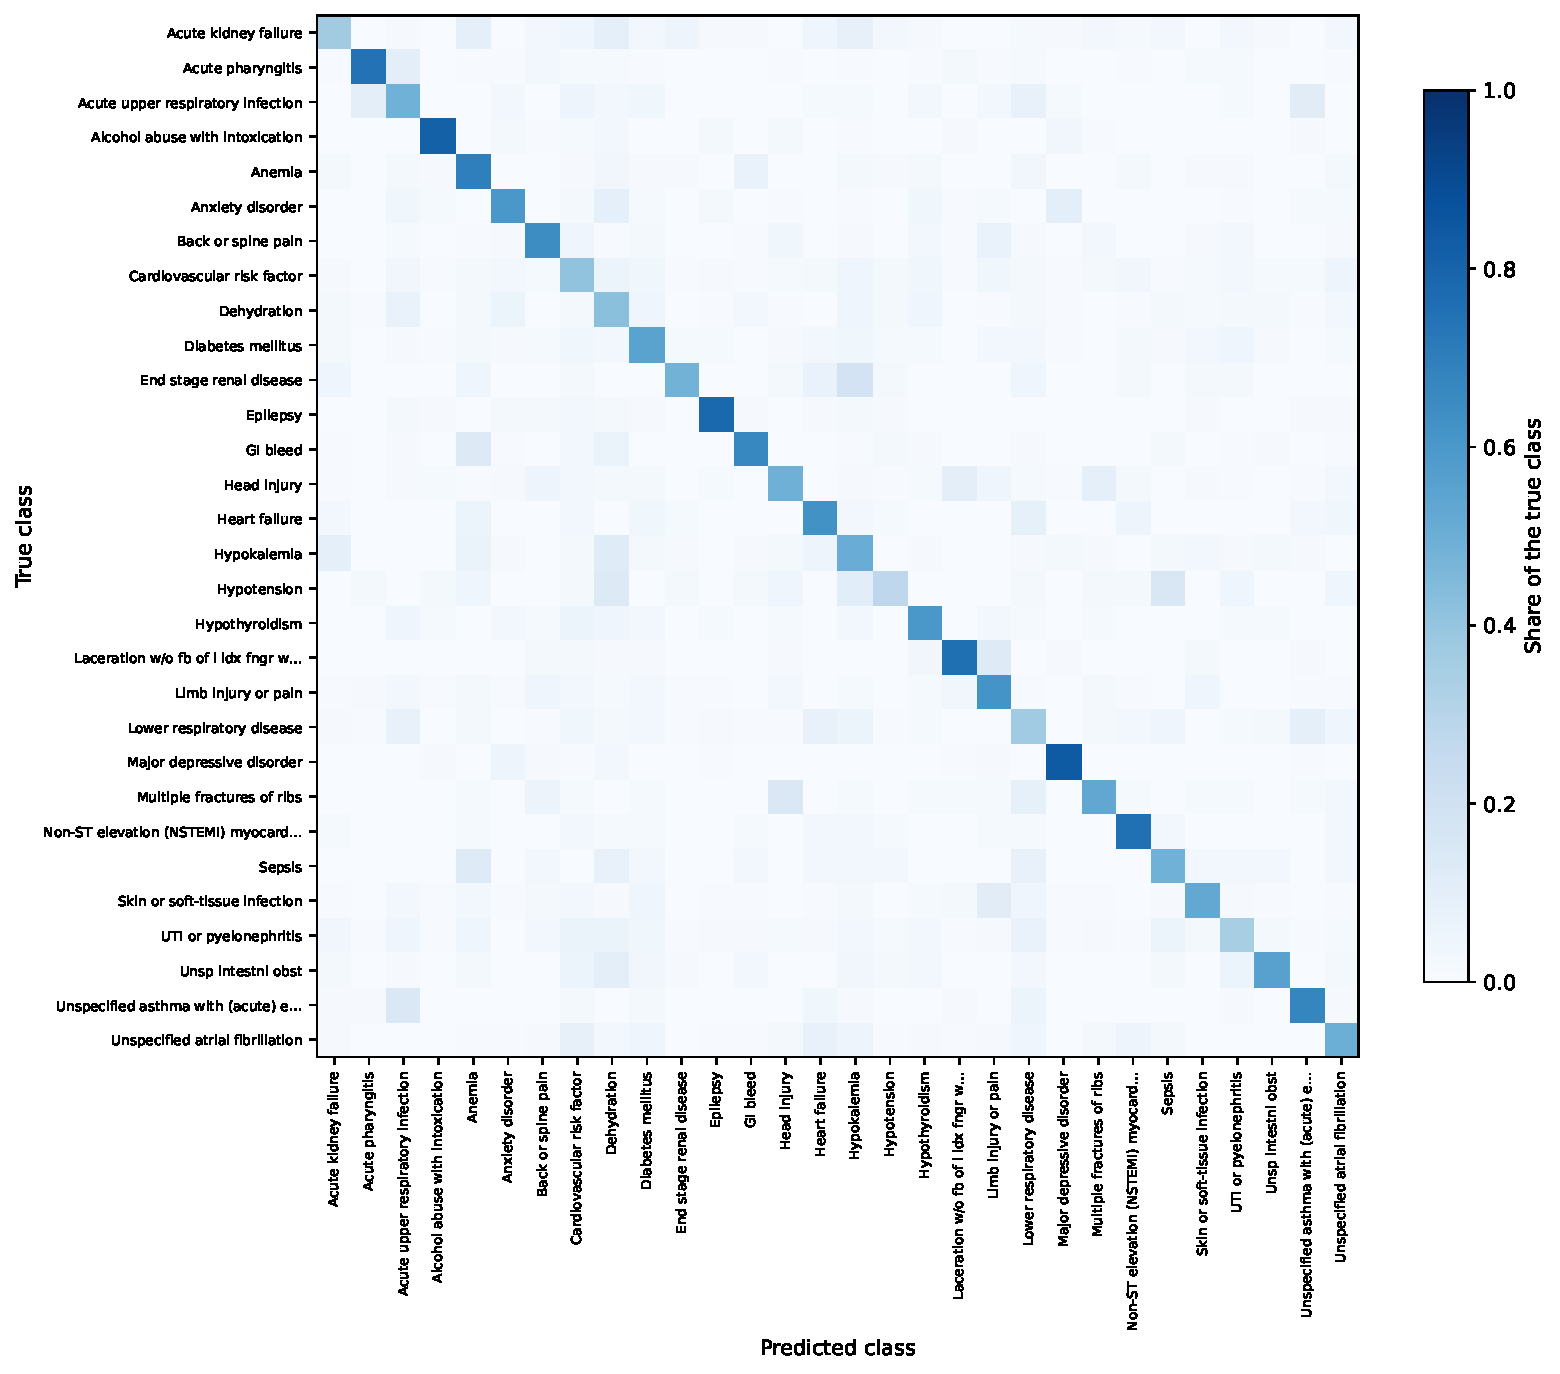
\includegraphics[width=\textwidth]{assets/confusion_matrix.pdf}
  \caption{Row-normalised confusion matrix for the prototype model on the
    canonical test fold (7,456 graphs, 30 classes). Rows are true classes,
    columns predicted classes; darker means a larger share of that true class.}
  \label{fig:confusion}
\end{figure}

\subsection{Explanation Quality}
\label{sec:expl-quality}

Because the clinical data has no ground-truth importance masks, explanation
quality is assessed through sparsity, inter-explainer agreement across the
three GraphXAI explainers, and the decoded clinical evidence
(Section~\ref{sec:eval-protocol}).

The explanation pass runs the three explainers on the first 50 graphs of the
canonical test fold, using the same checkpoint that produced the numbers in
Table~\ref{tab:main-results} (\texttt{comparison/\allowbreak
explain\_canonical.py}). Mean graph size is 21.7 nodes and 25 of the 50
predictions are correct, matching the overall test accuracy.

\caveat{\textbf{Sample size.} Unlike the predictive results, which cover the
full test fold of 7,456 graphs, every number in this section is computed on
those 50 graphs, that is 0.7\% of the test fold. The limit is GNNExplainer,
which optimises a separate mask per graph and needs several seconds per graph on
CPU, so explaining the full fold would take several hours. At $n = 50$ a
proportion such as the 32\% agreement reported below carries a 95\% confidence
interval of roughly $\pm 13$ percentage points, so the numbers below should be
read as the direction of an effect rather than as precise estimates. Every
statement in this section inherits that caveat.} \tbd{Re-run
\texttt{comparison/explain\_canonical.py --n 500} and update this section; at
$n = 500$ the same interval narrows to about $\pm 4$ points.} Sparsity is
measured as $1 - k/|V|$, where $k$ is the number of nodes carrying 90\% of the
total node-importance mass, so a higher value means the explanation concentrates
on fewer nodes. Table~\ref{tab:expl-quality} reports the results.

\begin{table}[htbp]
  \centering
  \caption{Explanation-quality summary across the three GraphXAI explainers,
    over 50 graphs of the canonical test fold \caveat{(0.7\% of it, not the full
    7,456; see the sample-size note in Section~\ref{sec:expl-quality})}. Sparsity is
    $1 - k/|V|$ at 90\% importance mass; higher means a more concentrated
    explanation. Top-node agreement is the share of graphs on which all three
    explainers rank the same node first.}
  \label{tab:expl-quality}
  \begin{tabular}{lcccc}
    \toprule
    Explainer & Mean sparsity & SD & Median & Top-node agreement \\
    \midrule
    GradExplainer            & 0.168 & 0.088 & 0.132 & \multirow{3}{*}{16/50 (32\%)} \\
    IntegratedGradExplainer  & 0.510 & 0.187 & 0.428 & \\
    GNNExplainer             & 0.563 & 0.146 & 0.550 & \\
    \bottomrule
  \end{tabular}
\end{table}

The three explainers behave differently on the same model. GNNExplainer and
Integrated Gradients concentrate the importance mass on roughly half of the
nodes, while the plain gradient explainer spreads it over almost the entire
graph: a ranking that needs 18 of 22 nodes to carry 90\% of the mass is not
something a clinician can act on.

The agreement numbers are the more informative result. All three explainers pick
the same most important node on 16 of the 50 explained graphs (32\%; \caveat{every
count in this paragraph is out of those 50, not out of the 7,456-graph test
fold}). Pairwise the rates
are similar, 52\% for the gradient explainer and GNNExplainer, 48\% for the
gradient explainer and Integrated Gradients, and 46\% for Integrated Gradients
and GNNExplainer, so no pair agrees on even two thirds of the graphs. Measured
on the top four nodes instead of the single top node, the mean overlap falls to
between 0.30 and 0.35, meaning about one of the four selected clinical factors
is shared.

This has a direct consequence for the interpretability claim. If three post-hoc
explainers applied to one fixed model disagree on which clinical entity drove
the prediction in two thirds of the cases, a single post-hoc attribution cannot
be presented as \emph{the} explanation of that prediction. The result is
consistent with the concern raised in~\cite{agarwal2023graphxai} that post-hoc
explanation quality degrades once graphs become larger and denser than the
synthetic benchmarks these methods were tuned on.

The intrinsic evidence behaves better on both counts, \caveat{on the same
50-graph sample}. The class of the nearest prototype matches the predicted class on 39 of
the 50 graphs, so the prototype layer is not decorative: it is largely what the
classifier reads. The distance
to that prototype also separates correct from incorrect predictions, averaging
0.122 when the prediction is right and 0.191 when it is wrong, which turns the
prototype evidence into a rough confidence signal that the post-hoc scores do
not provide. Because the prototypes are projected onto real training subgraphs,
that evidence is also traceable to actual patients rather than to a
reconstructed mask.

Read qualitatively, and \caveat{again over the same 50 graphs}, the decoded factors mix
clinically plausible and clinically empty signals. In a correctly predicted
finger laceration, the gradient
explainer and Integrated Gradients both rank \texttt{cc[laceration]} at the top
and the nearest three prototypes all belong to that class. Against that,
GNNExplainer ranks the patient demographic node (gender, race, transport mode)
first on most graphs, which carries no diagnostic content and mostly reflects
that the hub node aggregates the whole graph. The failure cases show the same
mechanism from the other side: a visit with an oxygen saturation almost five
standard deviations below the mean is predicted as hypokalaemia, with the
explainers pointing at a rash complaint and the patient's antiepileptic
medication instead of at the vital sign. Worked examples are given in
Appendix~\ref{app:results}.

%===============================================================
\section{Summary}
\label{sec:eval-summary}
%===============================================================

The evaluation gives three results.

On predictive performance, the tabular XGBoost baseline is the strongest model
on all six metrics (65.4\% accuracy, 0.607 macro-F1), ahead of GraphCare
(57.8\%, 0.470), the plain-GCN ablation (56.5\%, 0.516) and the prototype model
(56.3\%, 0.508). Since all four see the same clinical fields and the same test
patients, the intra-patient graph structure used here does not add predictive
information beyond what gradient-boosted trees extract from the flat feature
vector. Among the graph models the ordering depends on the metric: GraphCare
leads on overall accuracy and top-$k$ ranking, the prototype model and the
ablation on rare-class sensitivity, where both reach a balanced accuracy near
0.57 against 0.45 for GraphCare.

On the cost of interpretability, the ablation puts a number on the prototype
layer: removing it and keeping everything else fixed changes accuracy by 0.2
percentage points and macro-F1 by 0.008, in favour of the plain head. At that
size the self-explainable head is effectively free on this dataset, which is the
more useful version of the interpretability-performance trade-off than the one
usually assumed.

On explanation quality, \caveat{measured on a 50-graph sample rather than on the
full test fold}, the three post-hoc explainers disagree with each other more than they
agree: they pick the same most important node on 32\% of the explained graphs,
and their top-4 selections overlap by 0.30 to 0.35. Any single post-hoc
attribution is therefore a weak basis for a clinical claim. The intrinsic
evidence is more stable: the nearest prototype matches the predicted class on 39
of those 50 graphs and its distance separates correct from incorrect predictions
(0.122 versus 0.191), which supports the case for building the explanation into
the model rather than reconstructing it afterwards. \caveat{The gap between the
32\% explainer agreement and the 78\% prototype match is wide enough to survive
the sampling error at this size, but the individual figures are not precise
(Section~\ref{sec:expl-quality}).}

The per-class analysis adds a fourth, more clinical result: the model is
reliable on presentations with a distinctive complaint or medication signature
(alcohol intoxication, depression, pharyngitis, GI bleed, all above 0.73 F1) and
weak on states defined by laboratory values or systemic findings (hypotension,
UTI, acute kidney failure, all below 0.44 F1), which is where a decision-support
tool would need to be trusted least.

\tbd{Method~C has not been implemented, so its row in
Table~\ref{tab:main-results} and its row in Table~\ref{tab:positioning} remain
open, together with the per-class error analysis in
Section~\ref{sec:error-analysis}.}

\chapter{Summary and Conclusions}\label{conclusions}

\section{Conclusion}

\section{Limitations and Future Work}





\printbibliography[heading=bibintoc, title={Bibliography}]

\chapter*{Abbreviations}
\addcontentsline{toc}{chapter}{Abbreviations}
\markboth{ABBREVIATIONS}{}

\abr{AI}{Artificial Intelligence}
\abr{AUPRC}{Area Under the Precision-Recall Curve}
\abr{AUROC}{Area Under the Receiver Operating Characteristic Curve}
\abr{CE}{Cross-Entropy}
\abr{ED}{Emergency Department}
\abr{EHR}{Electronic Health Record}
\abr{GAT}{Graph Attention Network}
\abr{GCN}{Graph Convolutional Network}
\abr{GDPR}{General Data Protection Regulation}
\abr{GNN}{Graph Neural Network}
\abr{HPO}{Hyperparameter Optimisation}
\abr{ICD}{International Classification of Diseases}
\abr{MCTS}{Monte Carlo Tree Search}
\abr{MIMIC}{Medical Information Mart for Intensive Care}
\abr{MLP}{Multi-Layer Perceptron}
\abr{MPS}{Metal Performance Shaders}
\abr{PMI}{Pointwise Mutual Information}
\abr{PyG}{PyTorch Geometric}
\abr{ReLU}{Rectified Linear Unit}
\abr{XAI}{Explainable Artificial Intelligence}
\abr{XGBoost}{eXtreme Gradient Boosting}

% \input{chapters/glossary.tex}

\addcontentsline{toc}{chapter}{List of Figures}
\listoffigures

\addcontentsline{toc}{chapter}{List of Tables}
\listoftables

\appendix

\chapter{Results}\label{app:results}

This appendix collects the detailed results that support Chapter~\ref{evaluation}.

\section{Per-Class Performance}

Table~\ref{tab:per-class} gives precision, recall, F1 and support for all 30
classes on the canonical test fold, for the prototype model
(\texttt{comparison/\allowbreak protgnn\_canonical}), sorted by support. It is
the detail behind the aggregate numbers in Table~\ref{tab:main-results} and the
error analysis in Section~\ref{sec:error-analysis}.

\begin{table}[htbp]
  \centering
  \small
  \setlength{\tabcolsep}{4pt}
  \caption{Per-class test performance of the prototype model on the canonical
    split. Macro-F1 is the unweighted mean of the F1 column (0.508).}
  \label{tab:per-class}
  \begin{tabular}{lrrrr}
    \toprule
    Diagnosis class & Precision & Recall & F1 & Support \\
    \midrule
    Limb injury or pain & 0.732 & 0.615 & 0.668 & 903 \\
    Back or spine pain & 0.820 & 0.644 & 0.722 & 855 \\
    Cardiovascular risk factor & 0.586 & 0.406 & 0.479 & 749 \\
    Head injury & 0.687 & 0.490 & 0.572 & 502 \\
    Diabetes mellitus & 0.584 & 0.551 & 0.567 & 425 \\
    UTI or pyelonephritis & 0.590 & 0.341 & 0.433 & 413 \\
    Skin or soft-tissue infection & 0.678 & 0.524 & 0.591 & 389 \\
    Lower respiratory disease & 0.464 & 0.366 & 0.409 & 369 \\
    Alcohol abuse with intoxication & 0.897 & 0.812 & 0.852 & 345 \\
    GI bleed & 0.810 & 0.666 & 0.731 & 302 \\
    Major depressive disorder & 0.832 & 0.835 & 0.834 & 267 \\
    Unspecified atrial fibrillation & 0.420 & 0.497 & 0.455 & 179 \\
    Acute pharyngitis & 0.828 & 0.744 & 0.784 & 168 \\
    Anxiety disorder & 0.497 & 0.601 & 0.544 & 138 \\
    Dehydration & 0.189 & 0.419 & 0.261 & 129 \\
    Acute kidney failure & 0.377 & 0.359 & 0.368 & 128 \\
    Hypokalemia & 0.266 & 0.504 & 0.348 & 127 \\
    Laceration w/o fb of l idx fngr w/o damage to nail & 0.449 & 0.754 & 0.563 & 122 \\
    Unsp intestnl obst & 0.591 & 0.556 & 0.573 & 117 \\
    Anemia & 0.325 & 0.693 & 0.443 & 114 \\
    Unspecified asthma with (acute) exacerbation & 0.481 & 0.670 & 0.560 & 112 \\
    Epilepsy & 0.608 & 0.784 & 0.685 & 97 \\
    Heart failure & 0.353 & 0.624 & 0.451 & 85 \\
    Acute upper respiratory infection & 0.175 & 0.488 & 0.257 & 82 \\
    Non-ST elevation (NSTEMI) myocardial infarction & 0.378 & 0.750 & 0.502 & 72 \\
    Multiple fractures of ribs & 0.223 & 0.529 & 0.314 & 70 \\
    Hypothyroidism & 0.236 & 0.600 & 0.339 & 65 \\
    Hypotension & 0.200 & 0.277 & 0.232 & 47 \\
    End stage renal disease & 0.404 & 0.477 & 0.438 & 44 \\
    Sepsis & 0.196 & 0.488 & 0.280 & 41 \\
    \bottomrule
  \end{tabular}
\end{table}

\section{Class Distribution}

The per-class counts for the canonical run are listed in
Table~\ref{tab:class-dist}, sorted by training frequency. The class names are
the merged disease categories used by the canonical split
(\texttt{comparison/\allowbreak canonical\_split.json}); earlier runs used the raw
\texttt{disease\_1} strings and are not comparable.

\begin{table}[htbp]
  \centering
  \small
  \caption{Class distribution for the 30-class disease dataset on the canonical
    split (train / validation / test).}
  \label{tab:class-dist}
  \begin{tabular}{lrrrr}
    \toprule
    Diagnosis class & Train & Share & Val & Test \\
    \midrule
    Limb injury or pain & 7{,}224 & 12.1\% & 903 & 903 \\
    Back or spine pain & 6{,}841 & 11.5\% & 855 & 855 \\
    Cardiovascular risk factor & 5{,}986 & 10.0\% & 748 & 749 \\
    Head injury & 4{,}016 & 6.7\% & 502 & 502 \\
    Diabetes mellitus & 3{,}395 & 5.7\% & 424 & 425 \\
    UTI or pyelonephritis & 3{,}298 & 5.5\% & 412 & 413 \\
    Skin or soft-tissue infection & 3{,}114 & 5.2\% & 389 & 389 \\
    Lower respiratory disease & 2{,}952 & 5.0\% & 369 & 369 \\
    Alcohol abuse with intoxication & 2{,}755 & 4.6\% & 344 & 345 \\
    GI bleed & 2{,}417 & 4.1\% & 302 & 302 \\
    Major depressive disorder & 2{,}141 & 3.6\% & 268 & 267 \\
    Unspecified atrial fibrillation & 1{,}428 & 2.4\% & 178 & 179 \\
    Acute pharyngitis & 1{,}346 & 2.3\% & 168 & 168 \\
    Anxiety disorder & 1{,}103 & 1.9\% & 138 & 138 \\
    Dehydration & 1{,}027 & 1.7\% & 128 & 129 \\
    Acute kidney failure & 1{,}025 & 1.7\% & 128 & 128 \\
    Hypokalemia & 1{,}012 & 1.7\% & 126 & 127 \\
    Laceration w/o fb of l idx fngr w/o damage to nail & 971 & 1.6\% & 121 & 122 \\
    Unsp intestnl obst & 940 & 1.6\% & 118 & 117 \\
    Anemia & 913 & 1.5\% & 114 & 114 \\
    Unspecified asthma with (acute) exacerbation & 894 & 1.5\% & 112 & 112 \\
    Epilepsy & 774 & 1.3\% & 97 & 97 \\
    Heart failure & 680 & 1.1\% & 85 & 85 \\
    Acute upper respiratory infection & 656 & 1.1\% & 82 & 82 \\
    Non-ST elevation (NSTEMI) myocardial infarction & 577 & 1.0\% & 72 & 72 \\
    Multiple fractures of ribs & 558 & 0.9\% & 70 & 70 \\
    Hypothyroidism & 515 & 0.9\% & 64 & 65 \\
    Hypotension & 381 & 0.6\% & 48 & 47 \\
    End stage renal disease & 346 & 0.6\% & 43 & 44 \\
    Sepsis & 322 & 0.5\% & 40 & 41 \\
    \midrule
    Total & 59{,}607 & 100.0\% & 7{,}448 & 7{,}456 \\
    \bottomrule
  \end{tabular}
\end{table}

\section{Example Explanations}

The three cases below come from the explanation pass over the canonical test
fold (\texttt{comparison/\allowbreak protgnn\_canonical/\allowbreak
graphxai\_summary.csv}). \caveat{That pass covers 50 graphs, 0.7\% of the test
fold, so these cases illustrate the mechanisms described in
Section~\ref{sec:expl-quality} rather than establishing how often each one
occurs.} They were chosen to show one correct prediction with coherent evidence,
one failure where the model reads the wrong node, and the relation between
prototype distance and correctness. Node labels are the decoded
clinical tokens: \texttt{cc[\ldots]} is a triage chief complaint,
\texttt{sym[\ldots]} a doctor-assigned symptom code, drug names are home or
ED-administered medications, and arrows give the z-scored direction of a vital
sign.

\paragraph{Case 1, correct prediction with coherent evidence (graph 2).}
Predicted and true class: \emph{Laceration w/o fb of l idx fngr w/o damage to
nail}; 17 nodes. Integrated Gradients ranks \texttt{cc[laceration]} first and the
gradient explainer ranks it second, behind the patient node. The three nearest
prototypes (\#56, \#55, \#54, distances 0.074 to 0.076) all belong to the
predicted class, so the case-based evidence and the attribution point the same
way. GNNExplainer, as on most graphs, ranks the demographic hub node first and
then vital signs, which says little about the diagnosis.

\paragraph{Case 2, the model reads the wrong node (graph 5).}
Predicted \emph{Hypokalemia}, true class \emph{Lower respiratory disease}; 22
nodes. The visit carries an oxygen saturation 4.8 standard deviations below the
mean, flagged abnormal, which is the signal for the true class. The gradient
explainer does surface it, but only after \texttt{cc[rash]} and the patient node;
Integrated Gradients drops it entirely in favour of levetiracetam and
lamotrigine, the patient's antiepileptic medication. The nearest prototype is
\#46 (\emph{Hypokalemia}) at distance 0.173, and the next two are also
hypokalaemia prototypes, so the model is confidently matching the wrong
archetype. The explanation is faithful, it shows what the model used, but what
the model used was the medication history rather than the vital sign.

\paragraph{Case 3, prototype distance as a confidence signal (graph 0).}
Predicted and true class: \emph{GI bleed}; 17 nodes. The nearest prototype is
\#38 at distance 0.032, the closest match in the sample, with the next two
prototypes of the same class at 0.054 and 0.058. Integrated Gradients selects
\texttt{cc[rectal pain]} first, which is the presenting complaint for this
diagnosis. This is the pattern behind the aggregate numbers in
Section~\ref{sec:expl-quality}: tight prototype distances (mean 0.122 \caveat{over
the 50 explained graphs}) go with correct predictions, while the loose matches (mean
0.191) are where the model fails, as in Case 2.


\end{document}